\chapter{Hexagon Dataset
    \label{chapter:dataset}}
Most of the information for this chapter was taken from Lia Winklers master thesies.
The dataset was collected using the terrestrial laser scanner RTC 360 from Leica at 32 different locations.
In total, this dataset consists of 821 clean images and the number of images per location ranges from 4 to 423.
All the images are 360-degree panoramas with a
resolution of 8192 \(\times\) 4096 pixels.
The images are divided into the following 5 classes:

\begin{itemize}
    \item Indoor architectural
    \item Indoor construction
    \item Outdoor construction
    \item Outdoor Urban
    \item Forest
\end{itemize}

\noindent
To increase the accuracy of the algorithem the classes got rephrased and divided in subclasses.
These subclasses can be seen in \cref{tab:dataset:subclasses}.
\begin{table}[!ht]
    \centering
    \begin{tabular}{ccc}
    \toprule
    \textbf{1. Original}& \textbf{2. Rephrased}& \textbf{3. Subclasses}\\ \midrule
    Construction (in) & construction site & \makecell{construction site,\\ mining, tunnel}\\ \hline
    Architectural (in)& architectural& \makecell{architectural, office,\\ residential, school,\\ manufacturing, cellar,\\ laboratory} \\ \hline
    Construction (out)& construction site & construction site \\ \hline
    Urban (out)& town & \makecell{town, city,\\countryside, alley,\\ parking lot} \\ \hline
    Forest (out)& forest& forest \\
    \bottomrule
    \end{tabular}
    \caption{Rephrased terms and their subclasses
        \label{tab:dataset:subclasses}}
\end{table}

\begin{table}
    \centering
    \begin{tabular}{cc}
    \toprule
    \textbf{Class}& \textbf{Picture Classes}\\ \midrule
    Construction (in) & 9,13,39,12 \\ \hline
    Architectural (in)& 7,10,18,27,29,32,36,1,28,6,33,40,30,31,24\\ \hline
    Construction (out)& 8,16,22\\ \hline
    Urban (out)& 2,20,38,26,15,42,44,4,23\\ \hline
    Forest (out)& 17\\
    \bottomrule
    \end{tabular}
    \caption{Picture Classes of the hexagon dataset
        \label{tab:dataset:piccoding}}
\end{table}

The labels of the pictures are in the name of the picture.
The first number is the location where the picture was taken.
The second number is a sequential number for that location.
The \cref{tab:dataset:piccoding} tell you which class corresponds to which location.
For example the picture from \cref{fig:dataset:examplepic} is from the class Construction (in).

It is important to mention that the dataset is highly imbalanced.
Nearly 80\% of the panorama images are from the class indoor architectural.
This means that a "stupid" model can achieve a accuracy of 80\% by labeling every input as indoor architectural.
It is important to incoparate this fact in the evaluation of the performance of a model.

\begin{figure}
    \centering
    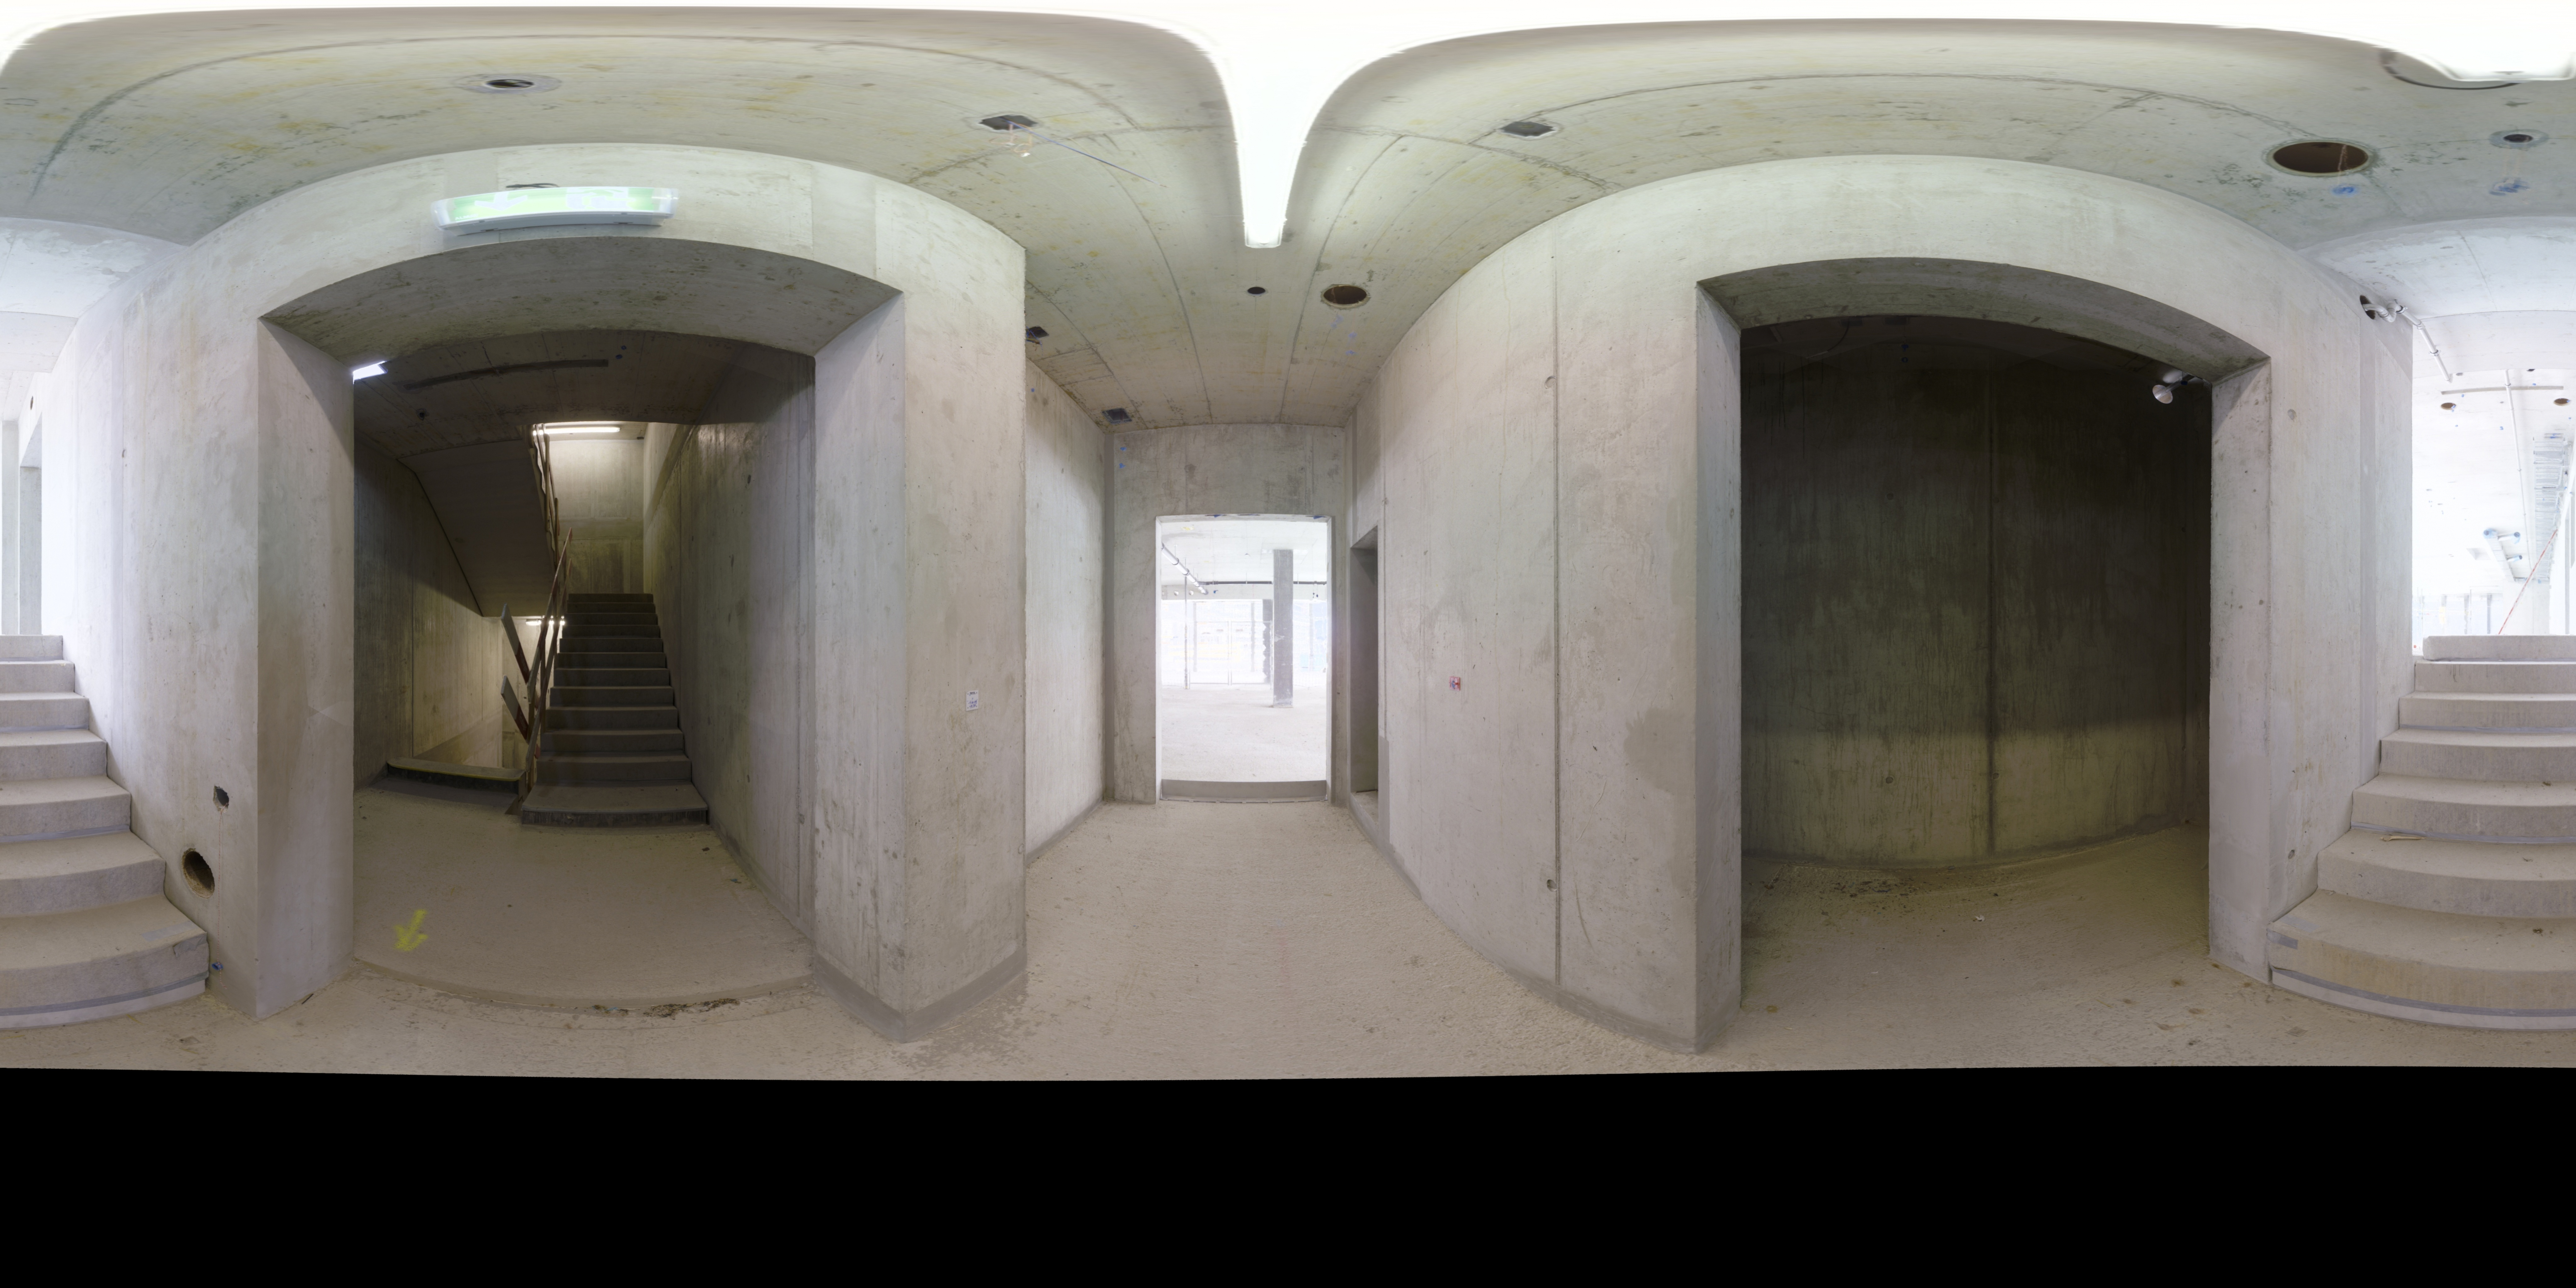
\includegraphics[width=\textwidth]{Images/Dataset/panorama_00009_0015.jpg}
    \caption{Example picture from the hexagon dataset [panorama\_00009\_0015.jpg]}
    \label{fig:dataset:examplepic}
\end{figure}

